
\documentclass[tikz,border=10pt]{standalone}
\begin{document}
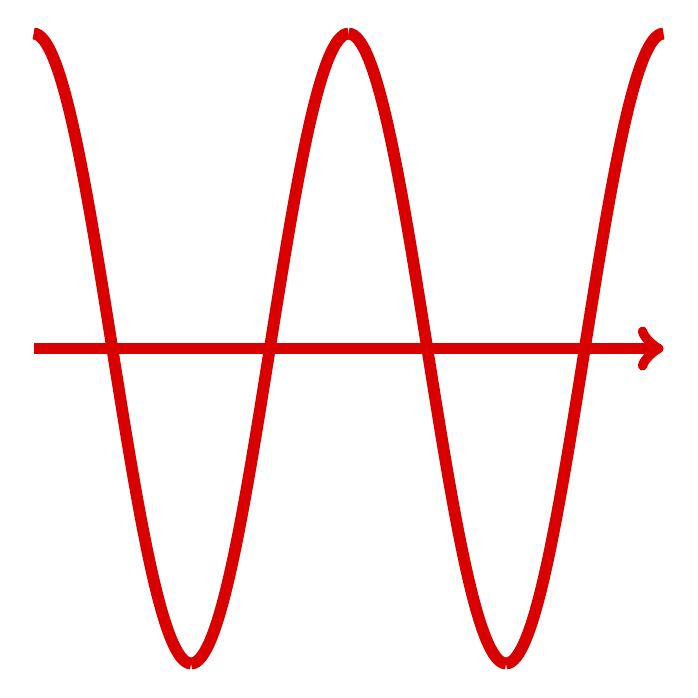
\begin{tikzpicture}
\draw[color=black!15!red,line width=1.5mm,->] (4,0) -- (12, 0);
\draw[color=black!15!red,line width=1.5mm]( 4, 4)  cos ( 5, 0);
\draw[color=black!15!red,line width=1.5mm]( 5, 0)  sin ( 6,-4);
\draw[color=black!15!red,line width=1.5mm]( 6,-4)  cos ( 7, 0);
\draw[color=black!15!red,line width=1.5mm]( 7, 0)  sin ( 8, 4);
\draw[color=black!15!red,line width=1.5mm]( 8, 4)  cos ( 9, 0);
\draw[color=black!15!red,line width=1.5mm]( 9, 0)  sin (10,-4);
\draw[color=black!15!red,line width=1.5mm] (10,-4) cos (11, 0);
\draw[color=black!15!red,line width=1.5mm] (11,0)  sin (12,4);
    \end{tikzpicture}

\end{document}
